% IMPORTANT: PLEASE USE XeLaTeX FOR TYPESETTING
\documentclass{sintefbeamer}
\usepackage{xeCJK}
\usepackage{amsthm}
\setbeamertemplate{theorems}[numbered]
\makeatletter
\setbeamertemplate{footline}
{
  \leavevmode%
  \hbox{%
  \begin{beamercolorbox}[wd=.7\paperwidth,ht=2.25ex,dp=1ex,center]{title in head/foot}%
    \usebeamerfont{title in head/foot} {IEEE Transactions on Knowledge and Data Engineering}
  \end{beamercolorbox}%
  \begin{beamercolorbox}[wd=.3\paperwidth,ht=2.25ex,dp=1ex,right]{date in head/foot}%
    \usebeamerfont{date in head/foot}\insertshortdate{}\hspace*{2em}
    \insertframenumber{} / \inserttotalframenumber\hspace*{2ex} 
  \end{beamercolorbox}}%
  \vskip0pt%
}

%\newtheorem{theorem}{Theorem} % to number according to section
\theoremstyle{definition}

\makeatother

% meta-data
\title{A Decentralized Federated Learning Framework via Committee Mechanism with Convergence Guarantee\\基于收敛保证下委员会机制的去中心化联邦学习框架}
\subtitle{汇报人:黄其涵 \qquad 导师:章静 教授 \qquad }
\author{IEEE Transactions on Parallel and Distributed Systems, 2022}
\date{\today}
\titlebackground{images/bg4}

% document body
\begin{document}

\maketitle


\section{Introduction}{}

\begin{frame}{1.1 Background}{Byzantine Generals Problem}
\begin{columns}
\begin{column}{0.35\textwidth}
\begin{figure}[ht]
\centering
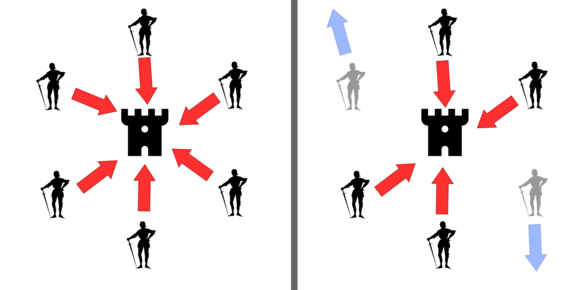
\includegraphics[width=1\textwidth]{images/Byzantine_Generals}
\end{figure}
\end{column}
\begin{column}{0.65\textwidth}
\textbf{拜占庭将军问题(Byzantine Generals Problem),是由莱斯利·兰波特中提出的分布式对等网络通信容错问题。}

在分布式计算中,不同的计算机通过通讯交换信息达成共识而按照同一套协作策略行动。但有时候,系统中的成员计算机可能出错而发送错误的信息,用于传递信息的通讯网络也可能导致信息损坏,使得网络中不同的成员关于全体协作的策略得出不同结论,从而破坏系统一致性。

%一组拜占庭将军分别各率领一支军队共同围困一座城市。为了简化问题,将各支军队的行动策略限定为进攻或撤离两种。因为部分军队进攻部分军队撤离可能会造成灾难性后果,因此各位将军必须通过投票来达成一致策略,即所有军队一起进攻或所有军队一起撤离。因为各位将军分处城市不同方向,他们只能通过信使互相联系。在投票过程中每位将军都将自己投票给进攻还是撤退的信息通过信使分别通知其他所有将军,这样一来每位将军根据自己的投票和其他所有将军送来的信息就可以知道共同的投票结果而决定行动策略。
\end{column}
\end{columns}
\end{frame}


\begin{frame}{1.1 Background}{Byzantine Attacks in FL}
\begin{columns}
\begin{column}{0.4\textwidth}
\begin{figure}[ht]
\centering
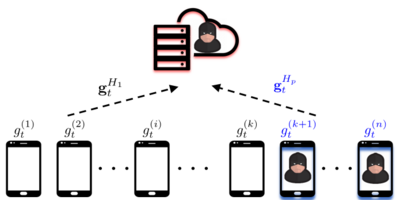
\includegraphics[width=1\textwidth]{images/bzt_fl}
\end{figure}
\end{column}
\begin{column}{0.6\textwidth}
\textbf{由于缺乏对本地梯度的身份认证,标准的联邦学习架构容易受到恶意客户端执行的拜占庭攻击。}主要分为以下两种类型的拜占庭攻击:
%标签翻转。攻击者将其训练数据的标签“翻转”为任意标签(例如,通过置换函数)。 • 添加噪音。攻击者通过添加噪声来降低模型质量来污染数据集。 • 后门触发器。攻击者将触发器注入原始数据集的一小块区域,导致分类器错误分类到目标类别中
\begin{itemize}
\item Training Data-based Attack (Label Flipping, Adding Noise, Backdoor Trigger)
\item Parameter-based Attack (Nonrandom Modification, Random Modification)
\end{itemize}
\end{column}
\end{columns}
\end{frame}

\begin{frame}{1.2 Contributions}
\begin{itemize}
\item \textbf{本文提出了一个去中心化的联邦学习框架CMFL,能够监控梯度聚合过程并防止恶意客户端和服务器阻碍全局模型的训练。}
\item \textbf{本文提出了一种选举策略和两种适用于不同场景的选择策略,可以保证算法的鲁棒性或加速训练过程。}
\item \textbf{本文给出了所提出的无服务器FL框架收敛性的证明和分析,作为理论保证,考虑了选举和选择策略对全局模型性能的影响。}
\item \textbf{本文通过实验结果表明,CMFL相比于比具有拜占庭容错的FL模型具有更快的模型收敛速度和更好的模型性能。}
\end{itemize}
\end{frame}

\section{Preliminaries}

\begin{frame}{2.1 Federated Learning}

\begin{columns}
\begin{column}{0.4\textwidth}
\begin{figure}[ht]
\centering
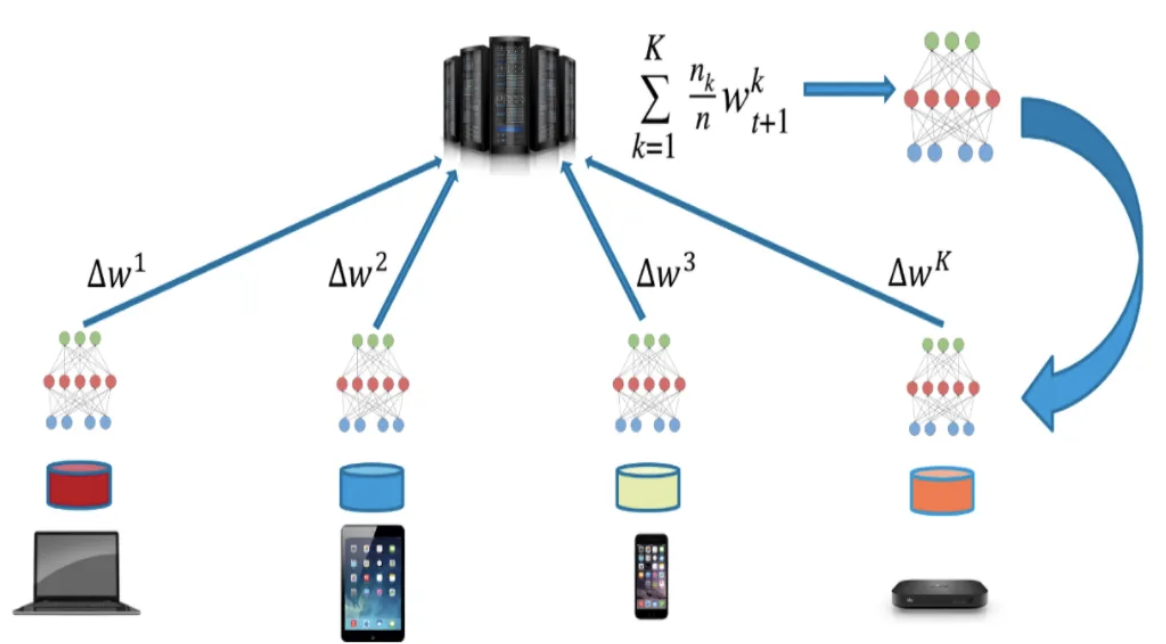
\includegraphics[width=1\textwidth]{images/fl_arch}
\end{figure}
\end{column}
\begin{column}{0.6\textwidth}
 在FL中服务器维护一个全局模型,每个客户端维护一个本地模型。在训练开始时,全局模型和所有本地模型将进行随机初始化,并在每轮通信中将执行以下步骤以完成训练过程:
\begin{itemize}
\item 服务器随机选择一部分客户端,然后将全局模型下载到本地;
\item 子集中的每个客户端执行一定数量的随机梯度下降;
\item 子集中的客户端将它们的本地梯度发送到服务器;
\item 服务器接收局部梯度并执行FedAvg算法以构建全局梯度,用于更新全局模型。
\end{itemize}
迭代直至算法收敛或模型精度满足要求。
\end{column}
\end{columns}
\end{frame}

\begin{frame}{2.2 Problem Formulation}

We consider the typical FL setup with total $K$ clients. The $k$ th client for $k=1, \ldots, K$ owns a local dataset $\mathcal{D}_k$, which contains $n_k=\left|\mathcal{D}_k\right|$ data samples. We denote the userdefined loss function for sample $\xi$ and model parameter vector $\mathbf{w}$ as $f(\mathbf{w}, \xi)$, the local objective function $F_k(\mathbf{w})$ on the $k$-th client can be written as follows:
$$
F_k(\mathbf{w})=\frac{1}{n_k} \sum_{\xi \in \mathcal{D}_k} f(\mathbf{w}, \xi) .
$$
We consider the following global objective function:
$$
F(\mathbf{w})=\sum_{k=1}^K p_k F_k(\mathbf{w})
$$
where $p_k=n_k / \sum_{k=1}^K n_k$ denotes the weight of the dataset on the $k$-th client. 
\end{frame}

\begin{frame}{2.2 Problem Formulation}
Formally, $\nabla F_k\left(\mathbf{w}_{k, i}^t\right)$ denotes the local gradient over dataset $\mathcal{D}_k$. Assume that at round $t$ the $k$ th client trains its local model $\mathbf{w}_{k, i}^t$ over mini-batch $\mathcal{B}_{k, i}^t$ for $i$ iterations of SGD, where $\mathcal{B}_{k, i}^t$ is randomly sampled from $\mathcal{D}_k$. Then the $k$-th client computes the local gradient $g_k\left(\mathbf{w}_{k, i}^t, \mathcal{B}_{k, i}^t\right)$ by the following formula:
$$
g_k\left(\mathbf{w}_{k, i}^t, \mathcal{B}_{k, i}^t\right)=\frac{1}{\left|\mathcal{B}_{k, i}^t\right|} \sum_{\xi \in \mathcal{B}_{k, i}^t} \nabla f\left(\mathbf{w}_{k, i}^t, \xi\right)
$$
The $g_k\left(\mathbf{w}_{k, i}^t, \mathcal{B}_{k, i}^t\right)$ is used to update the local model $\mathbf{w}_{k, i}^t$ as follows:
$$
\mathbf{w}_{k, i+1}^t=\mathbf{w}_{k, i}^t-\eta_i^t g_k\left(\mathbf{w}_{k, i}^t, \mathcal{B}_{k, i}^t\right)
$$
where $\eta_i^\iota$ represents the local learning rate at iteration $i$ of round $t$ and $\tau$ represents the maximal local SGD iterations. 

\end{frame}
\begin{frame}{2.2 Problem Formulation}
And after $\tau$ iterations of local updating, the local gradient $g_k\left(\mathbf{w}_{k, \tau}^t, \mathcal{B}_{k, \tau}^t\right)$ is sent to the server to construct a global gradient as follows:
$$
\bar{g}^t=\sum_{k \in S^t} p_{k, S^t} g_k\left(\mathbf{w}_{k, \tau}^t, \mathcal{B}_{k, \tau}^t\right),
$$
where $S^t$ denotes the subset of clients and $p_{k, S^t}=$ $n_k / \sum_{k \in S^t} n_k$ is the weight of the dataset on the $k$-th client of $S^t$. The $\overline{\mathbf{w}}^t$ is updated at each round as follows:
$$
\overline{\mathbf{w}}^{t+1}=\overline{\mathbf{w}}^t-\eta_t \bar{g}^t,
$$
where $\eta_t$ represents the global learning rate.
\end{frame}
\section{Methodology}

\begin{frame}{3.1 Framework of CMFL}
\centering
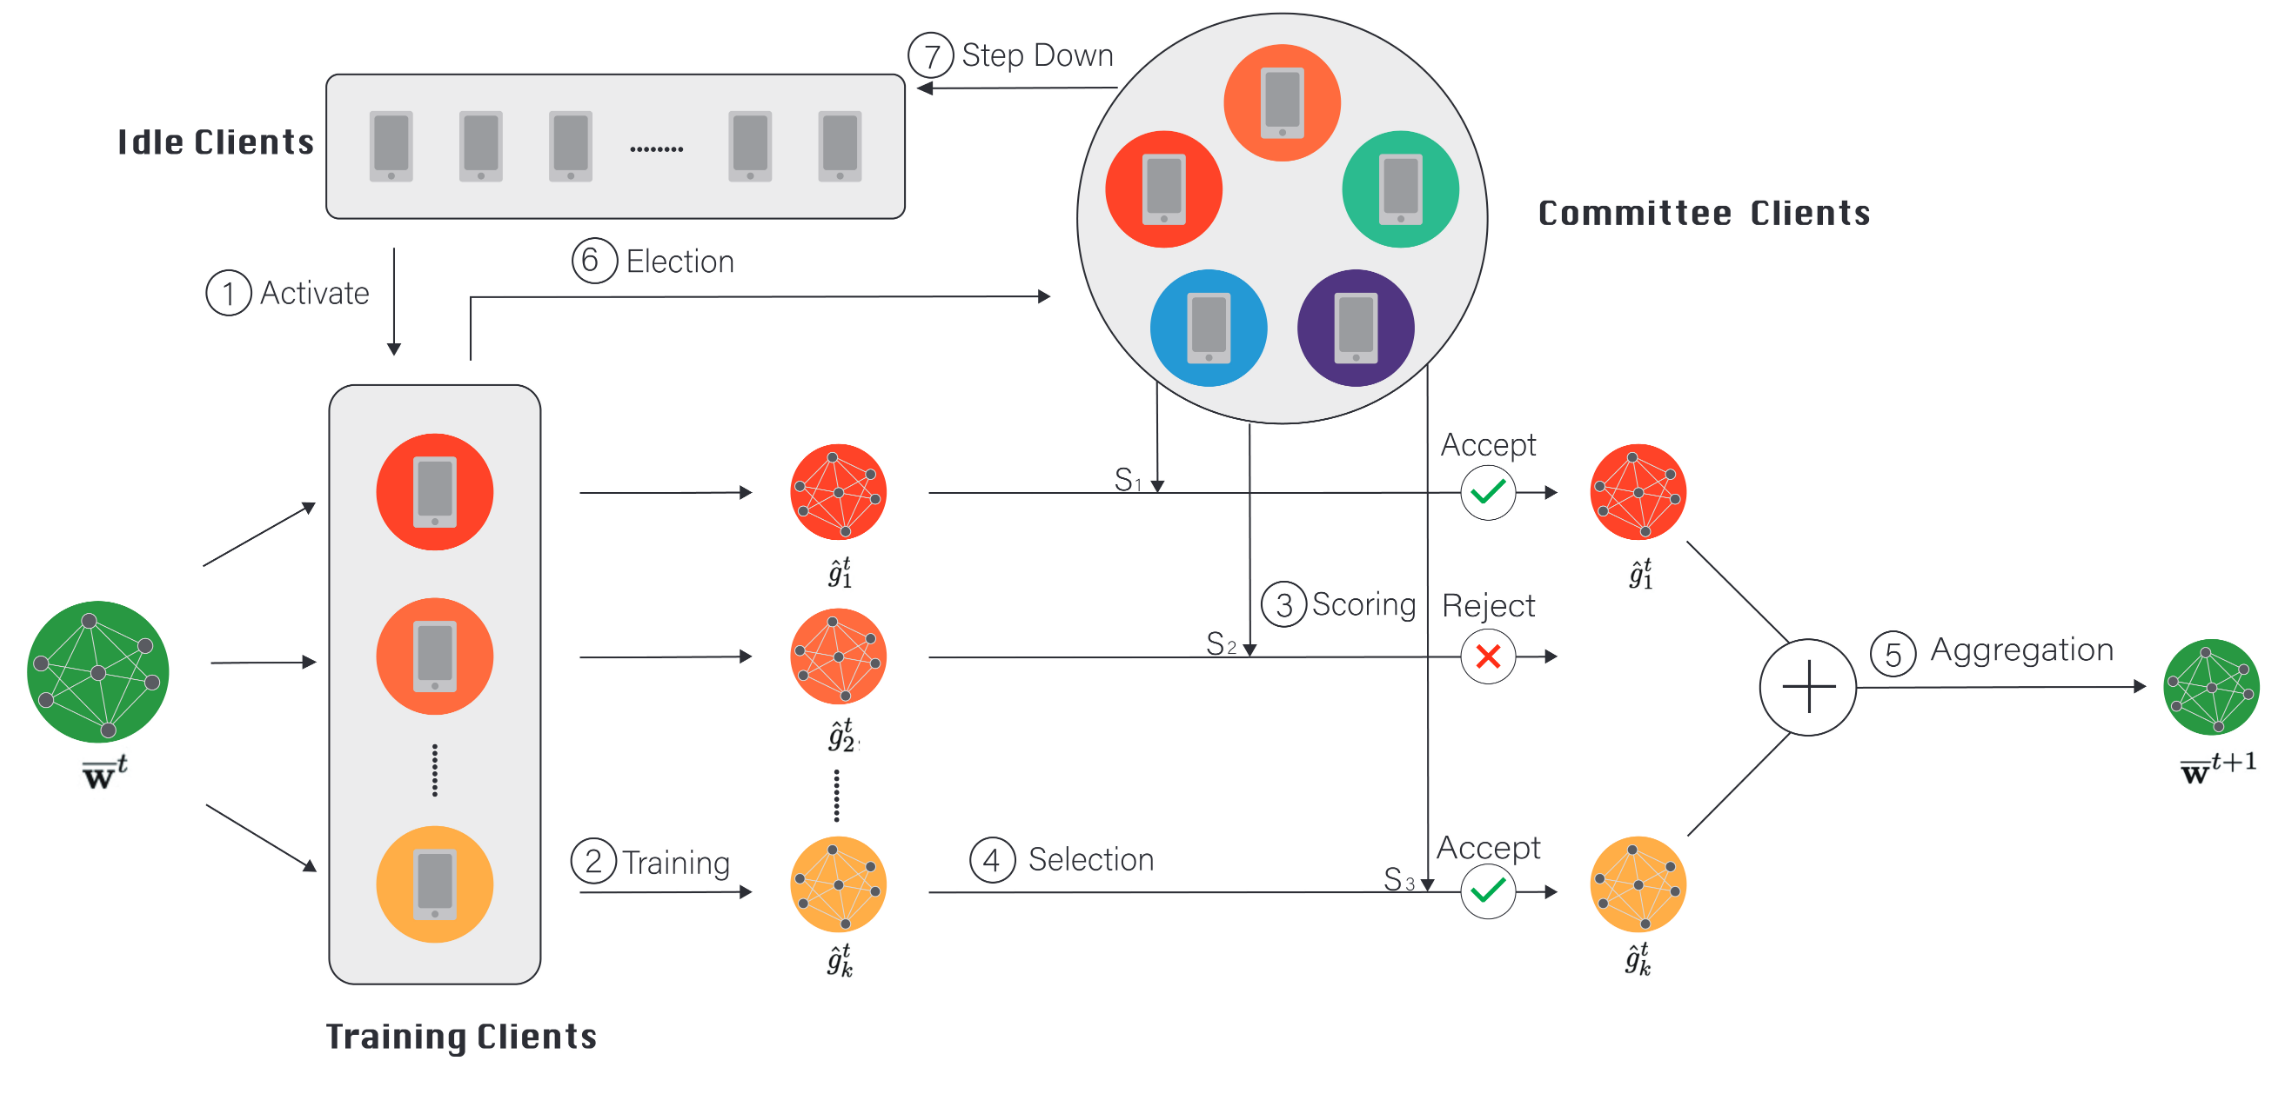
\includegraphics[width=1\textwidth]{images/cmfl_framework}

%图 1:CMFL 的训练过程如下: (1) 从空闲客户端中随机选择训练客户端; (2) training clients 和 committee clients 下载全局模型 wt 并开始训练,然后将它们的局部梯度 ^ gt k 发送给 committee clients; (3) 组委会客户根据评分系统为每位客户打分; (4) 委员会根据遴选策略遴选聚合客户; (5) 利用聚合客户端上传的局部梯度构建全局梯度wt+1; (6) 根据选举策略从培训客户中选出新的委员会客户; (7) 将上一轮的委员会客户添加到空闲客户列表中。
\end{frame}

\begin{frame}{3.2 Committee Mechanism}{Scoring System}
评分系统的关键是通过计算欧氏距离来区分诚实梯度和恶意梯度。两个诚实梯度的欧氏距离低于诚实梯度和恶意梯度的欧氏距离。基于这种认识,评分系统被设计为比较两个梯度的欧氏距离,其中上传诚实梯度的客户端可以获得更高的分数,而上传恶意梯度的客户端将获得较低的分数。
\\ \hspace*{\fill} \\
Assume that the local gradient on the $k$-th training client at round $t$ is denoted as $\hat{g}_k^t=g_k\left(\mathbf{w}_{k, \tau}^t, \mathcal{B}_{k, \tau}^t\right)$, and the local gradient on the the $c$-th committee client at round $t$ is expressed as $\hat{g}_c^t=g_c\left(\mathbf{w}_{c, \tau}^t, \mathcal{B}_{k, \tau}^t\right)$. The score $\mathcal{P}_k^c$ of the $k$ th training client assigned by the $c$-th committee client is computed as follows:
$$
\mathcal{P}_k^c=\frac{1}{\left\|\hat{g}_k^t-\hat{g}_c^t\right\|_2^2} .
$$
\end{frame}

\begin{frame}{3.2 Committee Mechanism}{Scoring System}
Since $\hat{g}_k^t$ and $\hat{g}_c^t$ are local gradients generated from different clients, we assume that $\hat{g}_k^t \neq \hat{g}_c^t$ for any $k \in S_b^t, c \in S_c^t$. We define 
$$
\mathcal{P}_k=\frac{1}{\frac{1}{C} \sum_c^C\left\|\hat{g}_k^t-\hat{g}_c^t\right\|_2^2}=\frac{C}{\sum_c^C \frac{1}{\mathcal{P}_k^c}}
$$
as the final score of the $k$-th training client. 
\\ \hspace*{\fill} \\
拜占庭攻击通常带有恶意梯度,这直接增加了这些梯度与诚实梯度之间的欧氏距离。因此,当恶意客户端的比例在可容忍范围内时,恶意训练客户端的分数预计会低于诚实训练客户端。但是,在没有拜占庭攻击的情况下,分数代表客户端的异构程度。得分越高意味着异质性程度越高。
\end{frame}

\begin{frame}{3.2 Committee Mechanism}{Selection Strategy}
基于上述 Scoring System 可以通过接受高分梯度来实现安全聚合,因为恶意梯度会获得低分。此外,收敛分析和实验结果表明,相反的策略在非攻击场景中表现更好。因此,针对不同的考虑,本文还设计了两种相反的选择策略如下:
\begin{itemize}
\item Selection Strategy I. 选择几个得分相对较高的局部梯度来构建全局梯度,用于全局模型的更新。此策略希望在欧几里德空间中类似于委员会梯度的局部梯度参与全局梯度的构建。
\item Selection Strategy II. 选择几个得分相对较低的局部梯度来构建全局梯度,用于全局模型的更新。此策略希望欧几里德空间中不同于委员会梯度的局部梯度参与全局梯度的构建。
\end{itemize}
\end{frame}

\begin{frame}{3.2 Committee Mechanism}{Election Strategy}
Election Strategy 旨在保证委员会客户的诚实。因此,委员会必须保证诚实的成员多于恶意的成员。否则,委员会无法过滤掉恶意梯度。本文根据分数对训练成员进行排序,然后选择这些靠近中间位置的训练成员作为下一轮的委员会成员。本文基于以下两个方面考虑来设计选举机制:
\begin{itemize}
\item \textbf{Robustness. } 恶意训练客户端会比诚实训练客户端获得更低的分数。因此,选择靠近中上位的训练客户端,可以防止恶意训练客户端成为下一轮的委员会客户端,从而保证全局模型的安全性。
\item \textbf{System Stability. } 得分最高的培训客户不会被选为新的委员会成员,以避免系统过于依赖委员会成员的初始化。即应符合“委员应该是能代表多数的人”的直觉。
%当我们选择那些得分最高的训练客户组成新的委员会时,全局模型的学习方向将完全由初始委员会成员决定。这是因为那些局部梯度与委员会梯度之间欧氏距离较大的客户,不仅难以被选中参与聚合过程,而且失去了竞选下一轮委员会成员的机会。这符合我们“委员应该是能代表多数的人”的直觉。
\end{itemize}


\end{frame}

\begin{frame}{3.2 Committee Mechanism}{Committee Consensus Protocol}
\begin{columns}
\begin{column}{0.5\textwidth}
\vspace{0.5em}
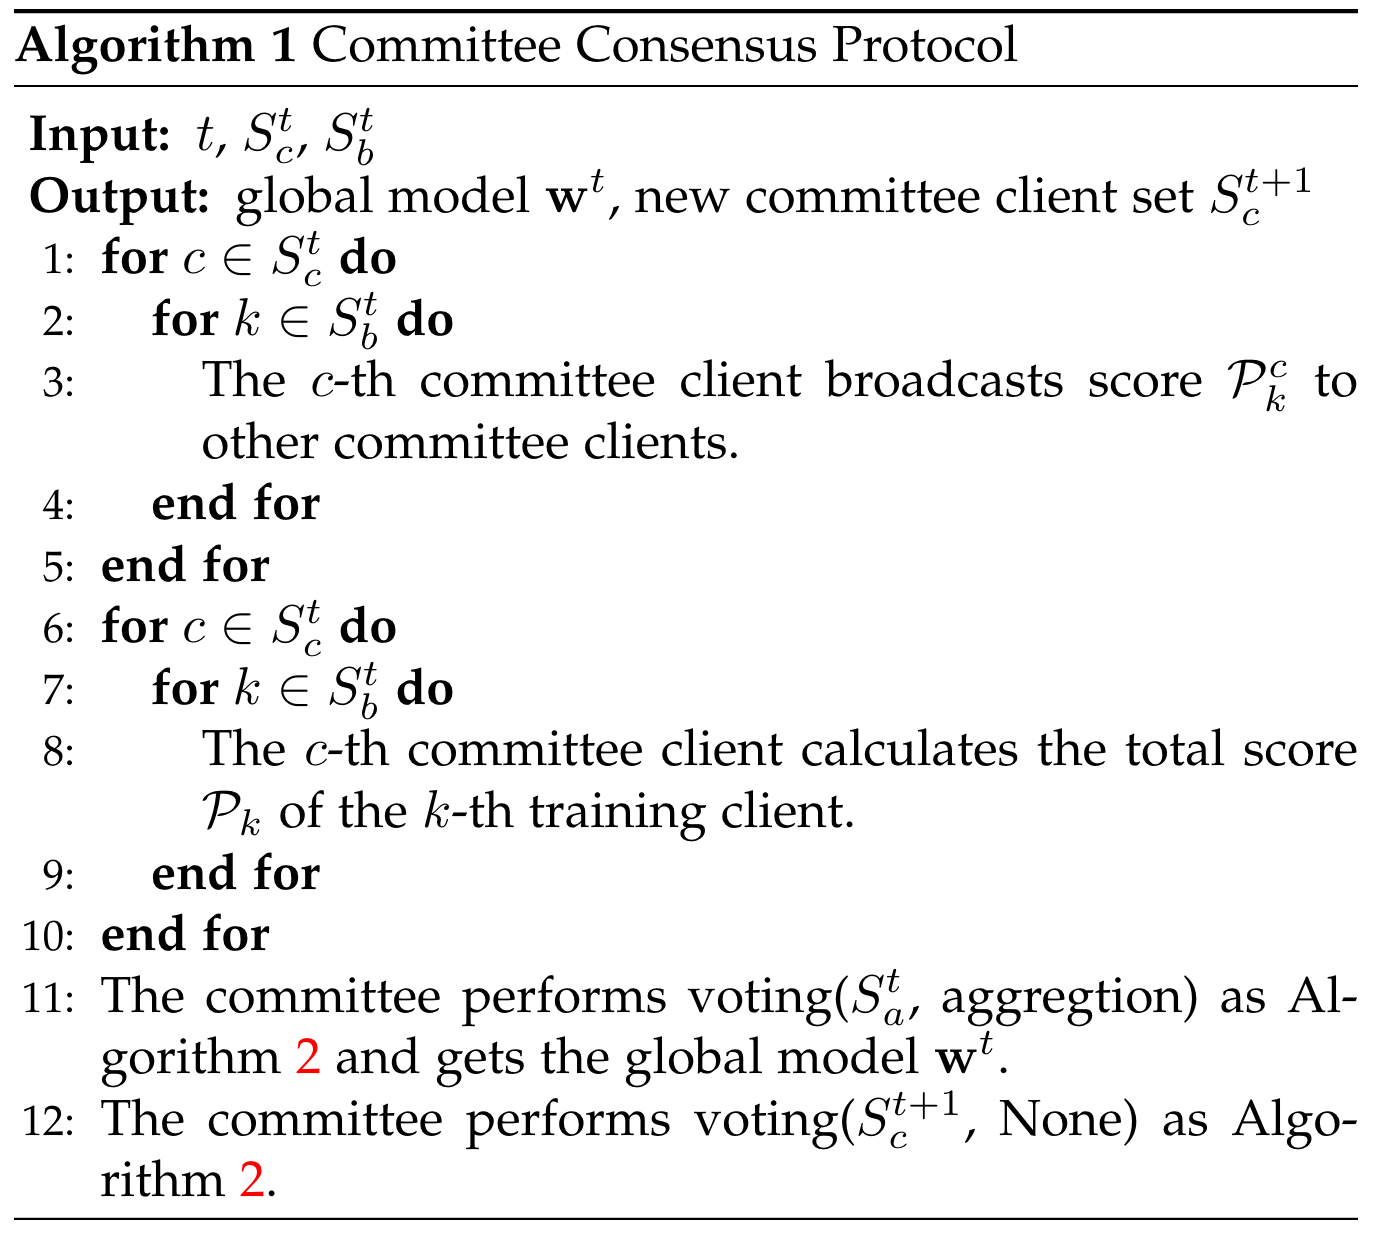
\includegraphics[width=1\textwidth]{images/algo_ccp}
\end{column}
\begin{column}{0.5\textwidth}
%在该去中心化框架中,委员会客户必须达成共识才能完成评分、聚合、选择和选举过程。
\\ \hspace*{\fill} \\
%The designed committee consensus protocol(CCP) is as follows(at round t):
%\begin{itemize}
%\item[1)] 评分过程结束后,每个委员会成员获得培训客户的分数。然后每个委员会成员将其分数广播给其他委员会成员。
%\item[2)] 随机选择一个委员会客户 p 作为主要委员会成员,而其他委员会成员被视为复制委员会成员。
%\item[3)] Gradient Verification.
%\item[4)] Global Model Updating.
%\item[5)] Election of New Committee Members.
%\end{itemize}
In our decentralized framework, the committee clients must reach a consensus to complete the scoring, aggregation, selection, and election process. Thus we design a committee consensus protocol, which is inspired by the pBFT
\end{column}
\end{columns}
\end{frame}

\begin{frame}{3.2 Committee Mechanism}{Committee Consensus Protocol - The Voting Algorithm}
\begin{columns}
\begin{column}{0.45\textwidth}
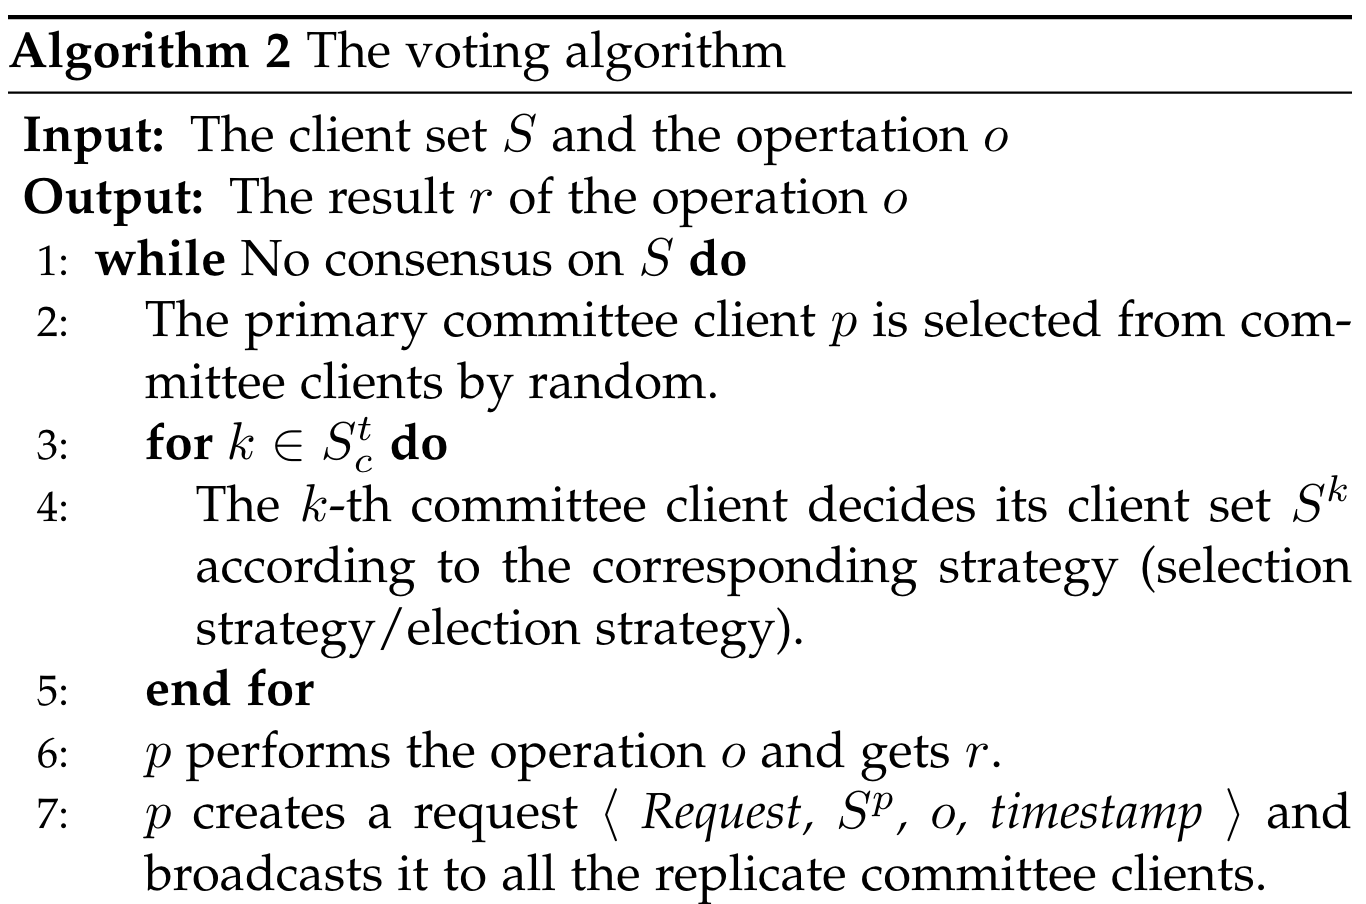
\includegraphics[width=1\textwidth]{images/algo_vote1}
\end{column}
\begin{column}{0.55\textwidth}
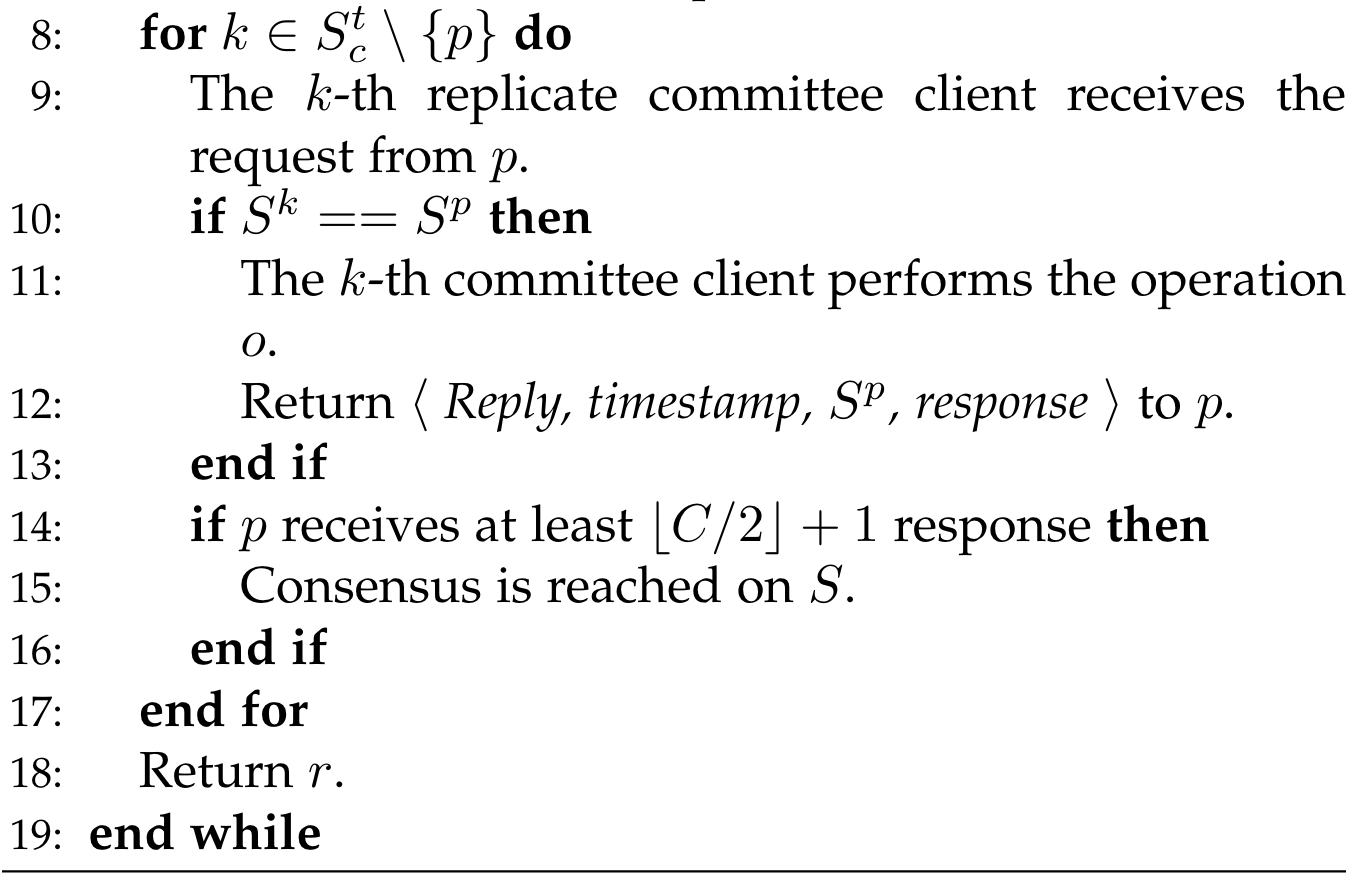
\includegraphics[width=1\textwidth]{images/algo_vote2}
\end{column}
\end{columns}
\end{frame}

\begin{frame}{3.3 Training Algorithm}
\begin{columns}
\begin{column}{0.5\textwidth}
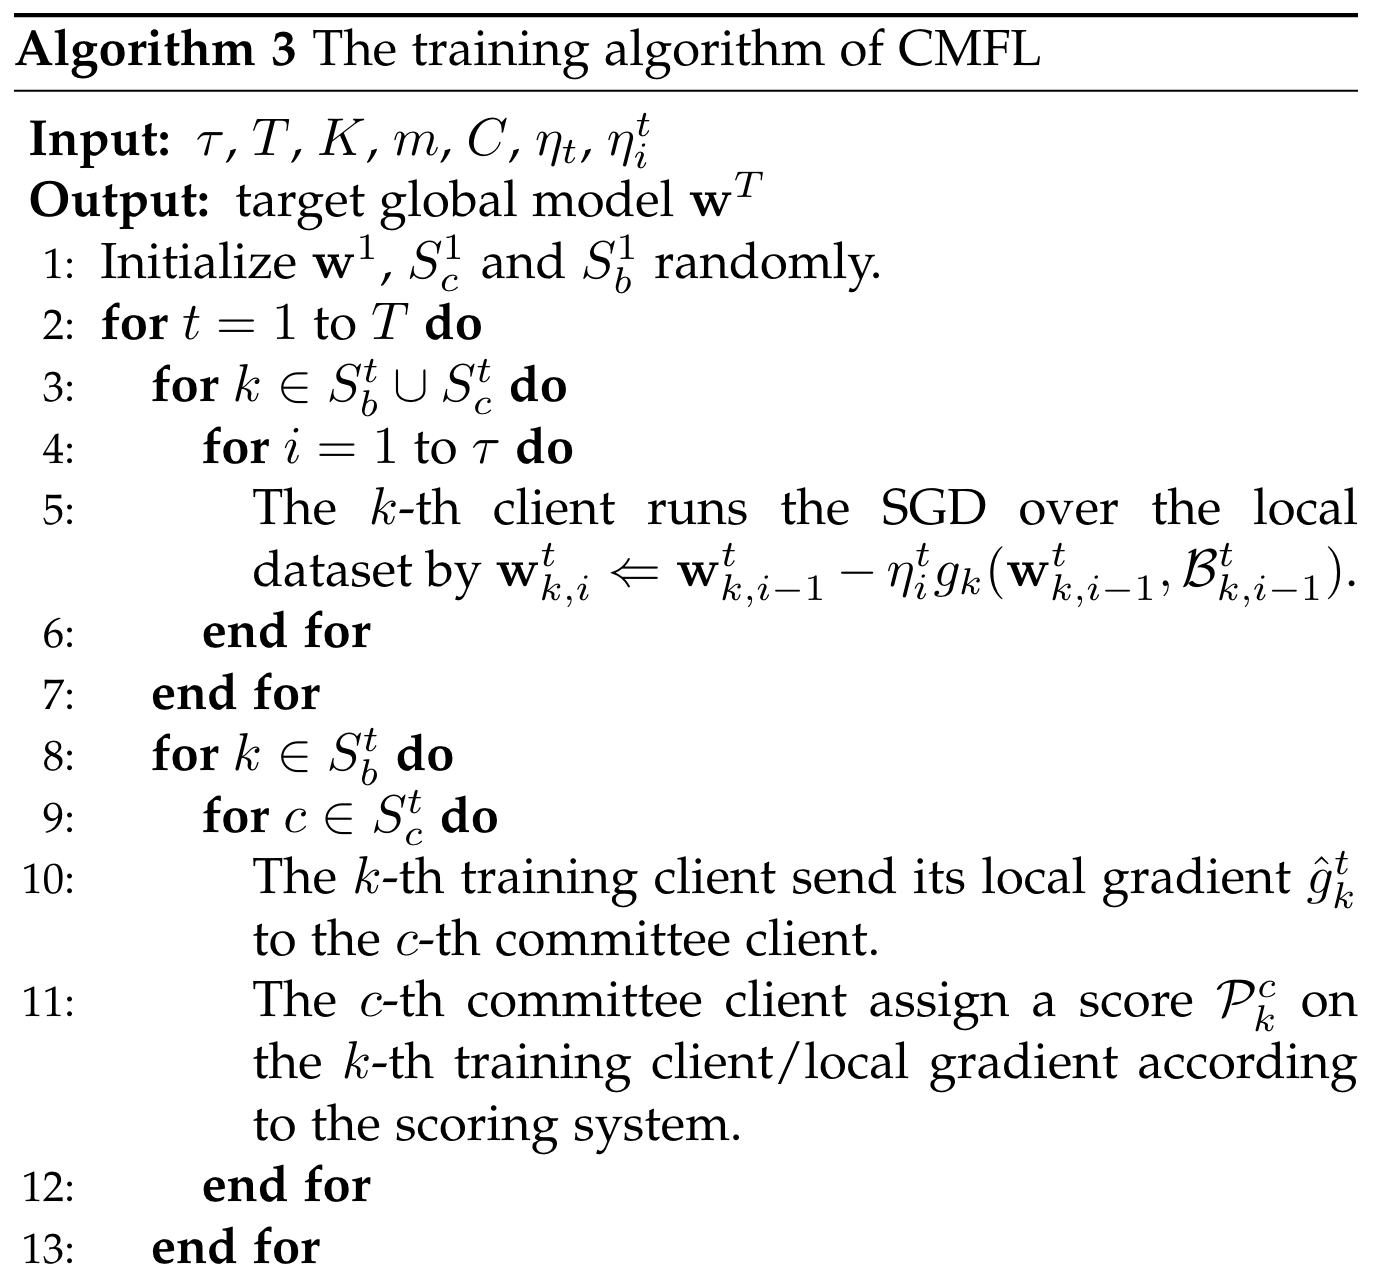
\includegraphics[width=0.95\textwidth]{images/algo_training1}
\end{column}
\begin{column}{0.45\textwidth}
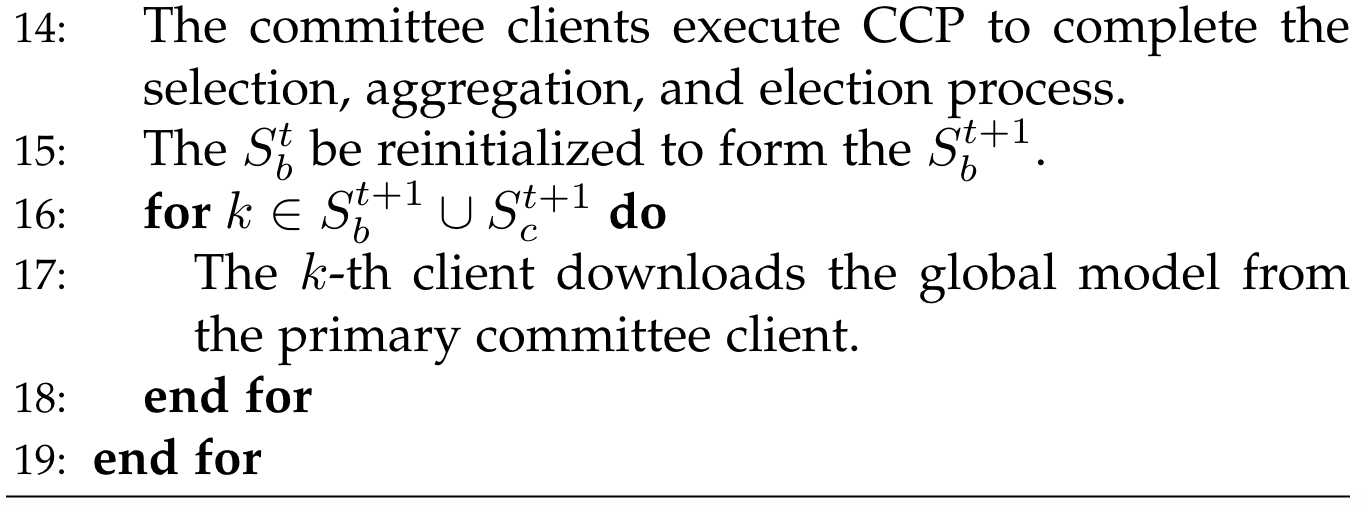
\includegraphics[width=0.95\textwidth]{images/algo_training2}

The algorithm performs the following five steps in each round:
\begin{itemize}
\item[1)] Random Sampling.
\item[2)] Local Training.
\item[3)] Gradient Verification.
\item[4)] Global Model Updating.
\item[5)] Election of New Committee Members.
\end{itemize}

\end{column}
\end{columns}
\end{frame}






\section{Experiments}

\begin{frame}{4.1 Nomal Training Experiment}{Experiment Setting}
	\begin{itemize}
\item[1)] FEMNIST-AlexNet. \textbf{FEMNIST} (Federated Extended MNIST) is a real-world distributed dataset formed by a specific division of the EMNIST dataset. 
\item[2)] Sentiment140-LSTM. \textbf{Sentiment140} is a realworld distributed dataset which focus on the text sentiment analysis task, including 1,600,000 tweets extracted using the Twitter API. 
\item[3)] Shakespeare-LSTM. \textbf{Shakespeare} is a real-world distributed dataset built from The Complete Works of William Shakespeare. 
\end{itemize}
\end{frame}

\begin{frame}{4.1 Nomal Training Experiment}{Result Analysis}
	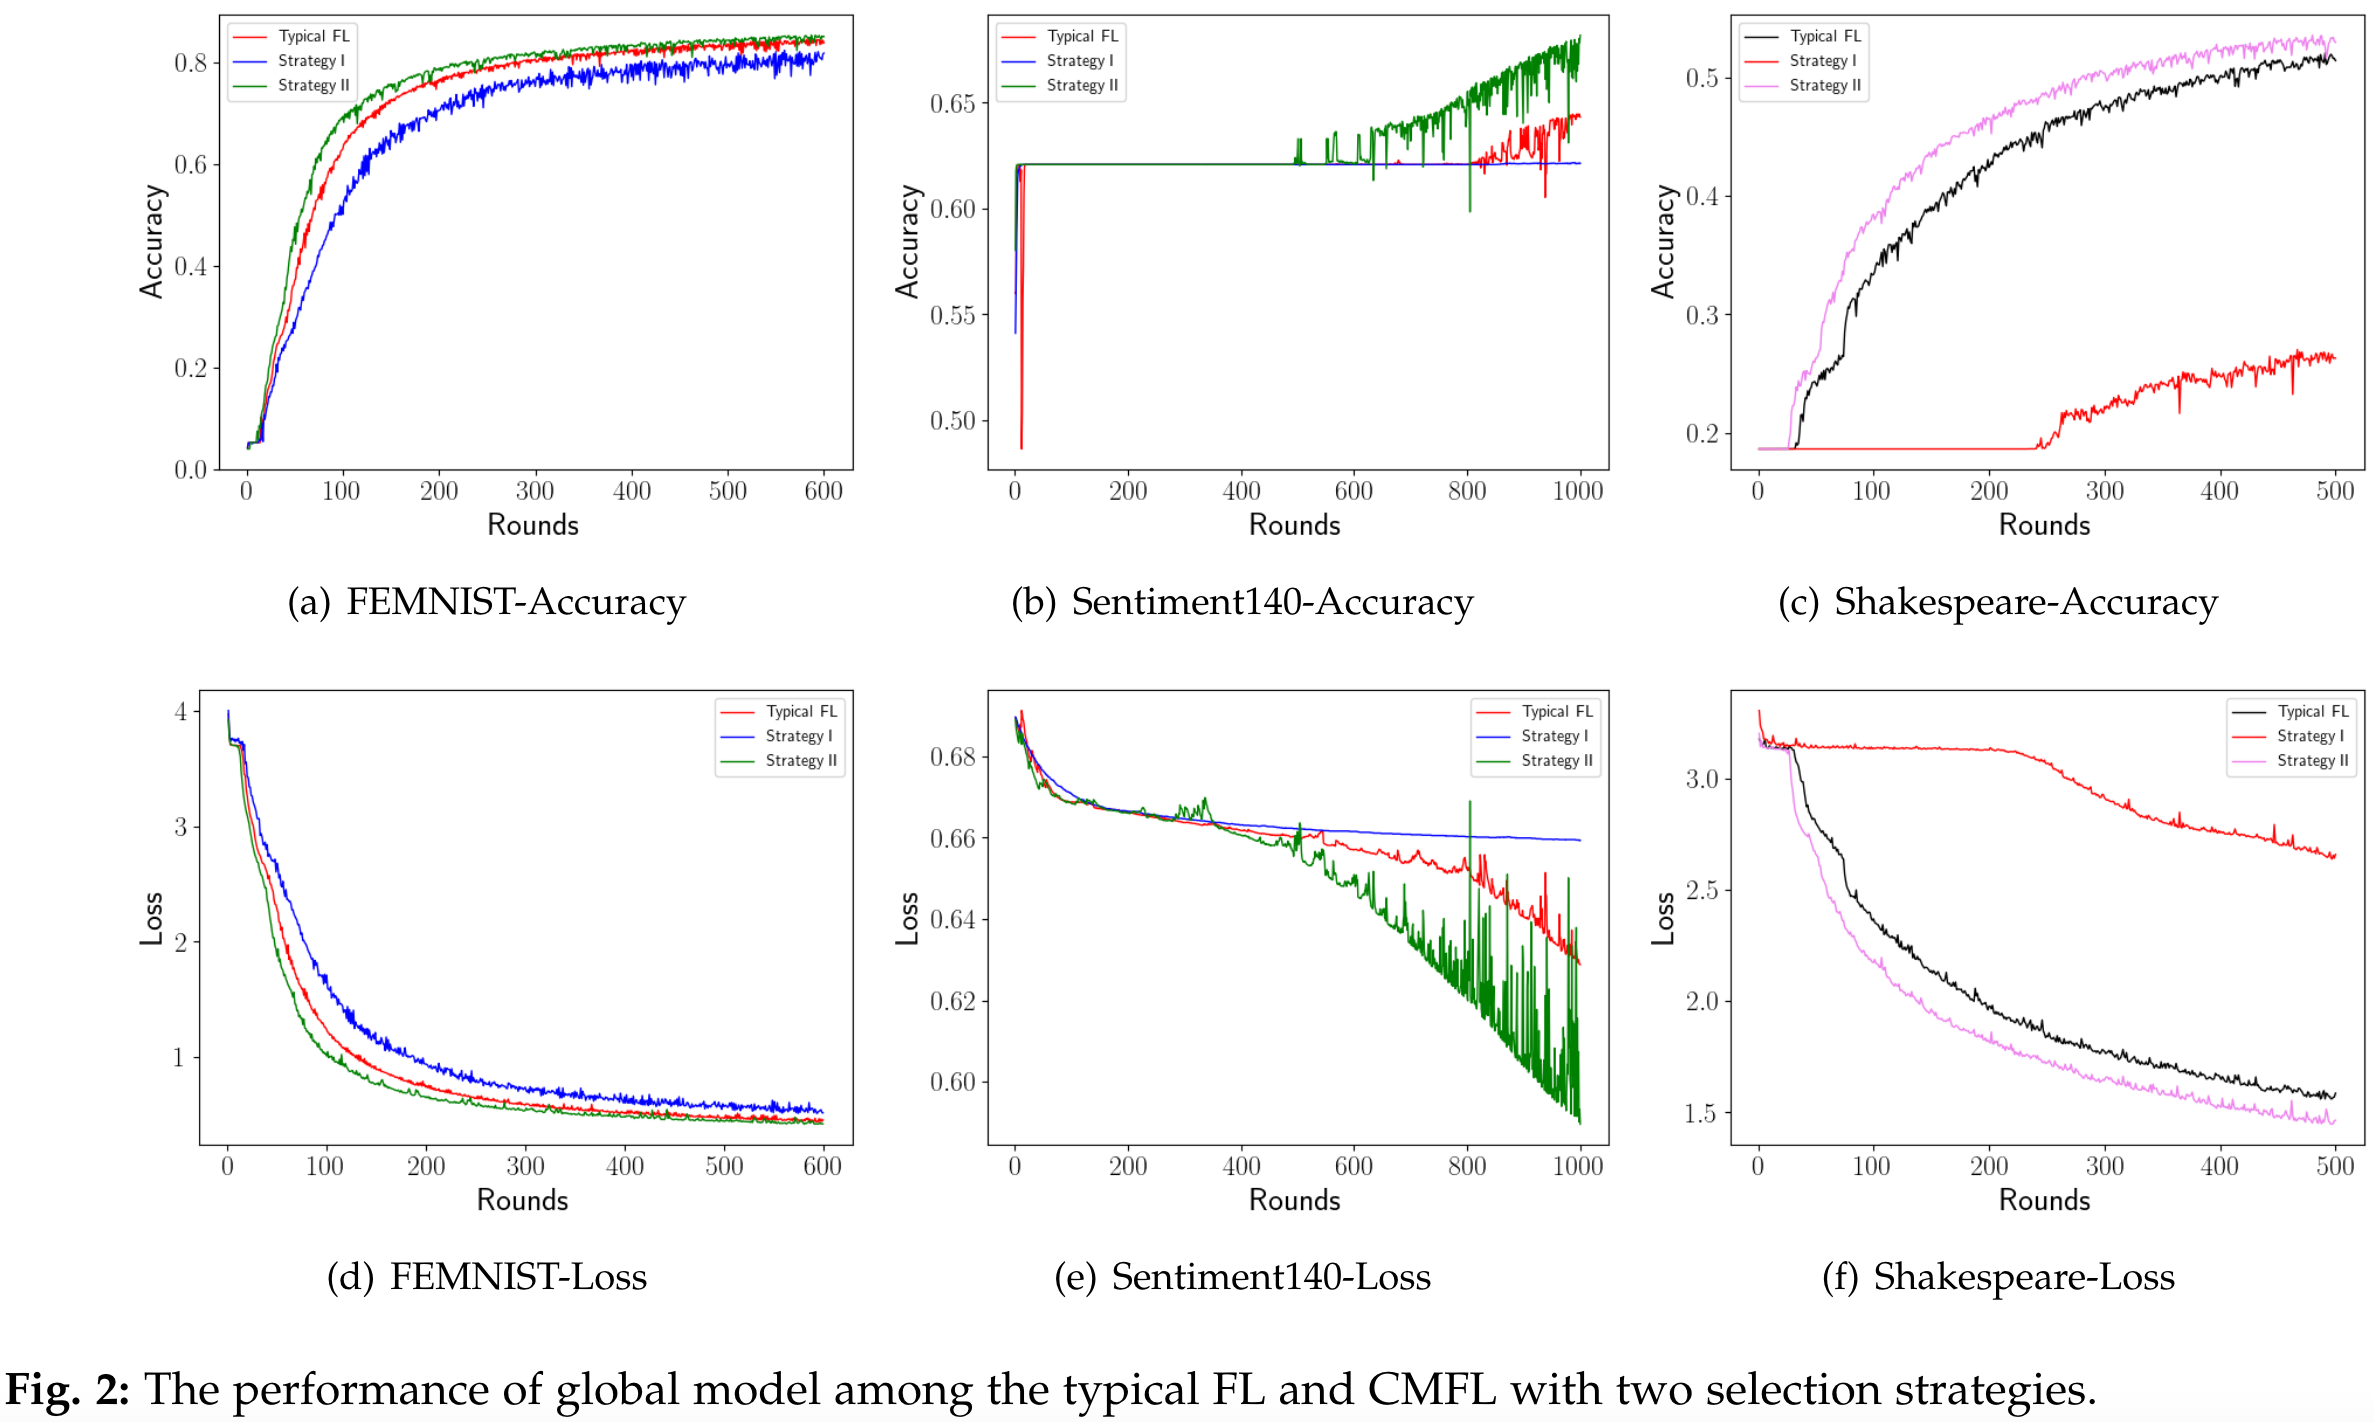
\includegraphics[width=0.78\textwidth]{images/exp_fig2}
\end{frame}

%\begin{frame}{4.2 Robustness Comparative Experiment}{Experiment Setting}
%	
%\end{frame}

%梯度缩放攻击:恶意客户端将局部梯度中的每个元素乘以一个随机值 λ ∈ [a, 1),其中 a 是一个定义的常数,表示攻击的强度。在这个实验中,我们设置 a = 0.5。 
%同值攻击:恶意客户端将局部梯度替换为大小相同且元素均为0 的向量。 
%反向梯度攻击:恶意客户端将局部梯度替换为向量大小相同方向相反。


\begin{frame}{4.2 Robustness Comparative Experiment}{Result Analysis}
	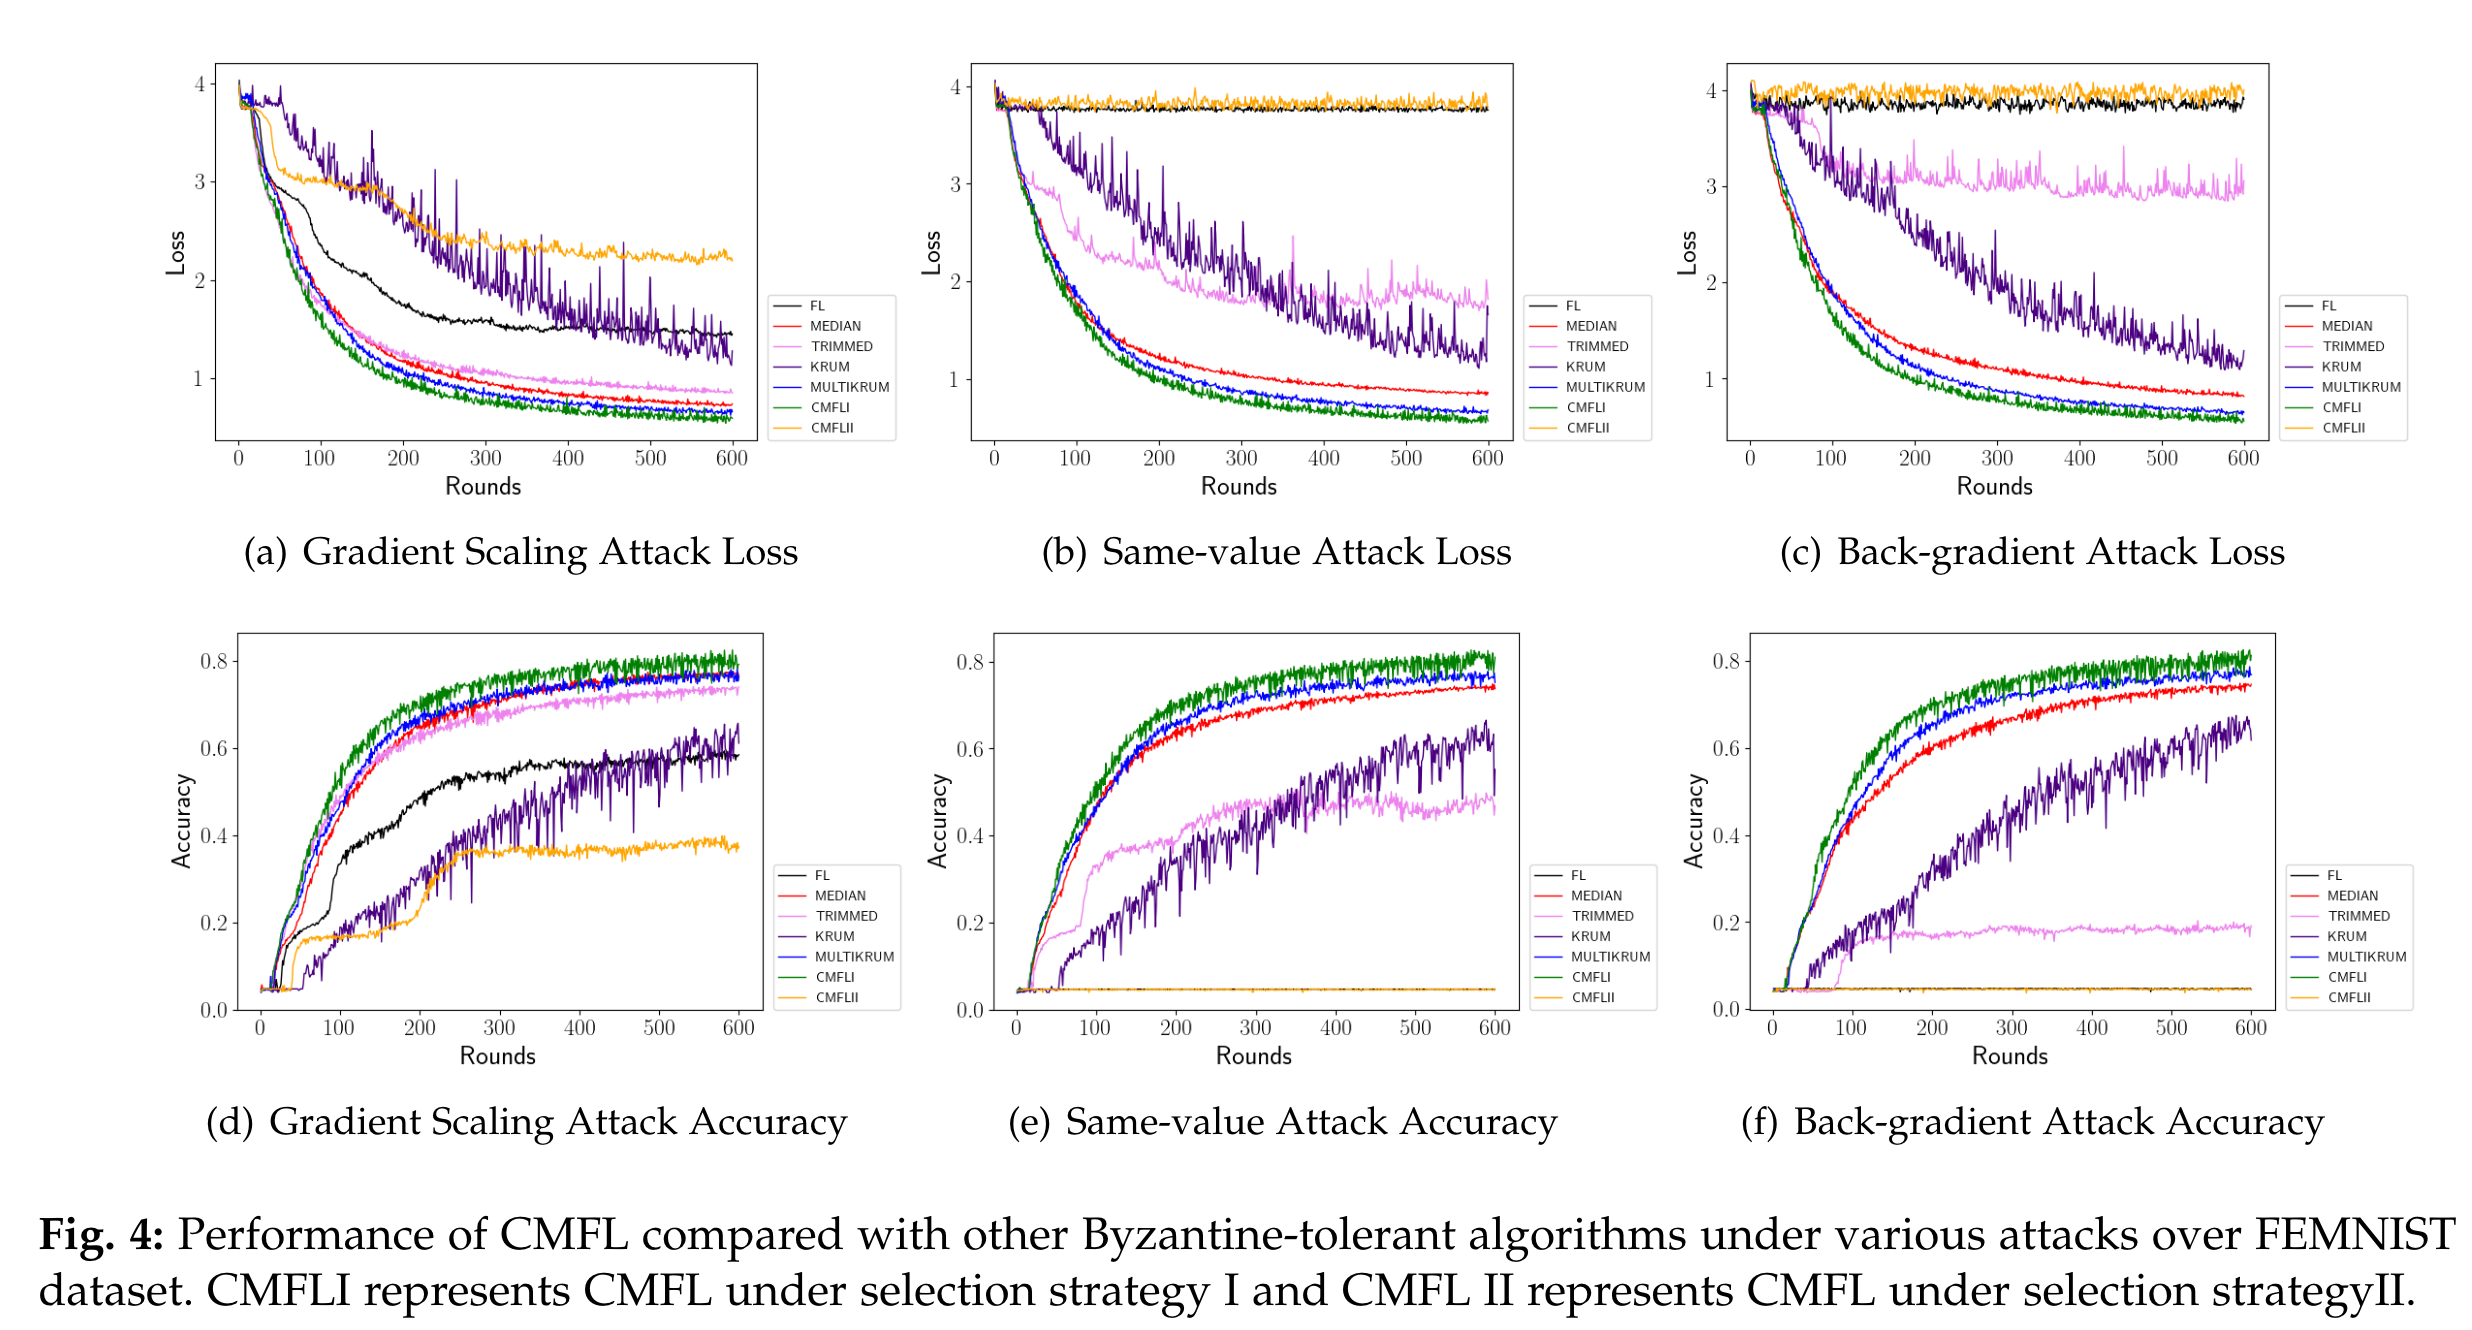
\includegraphics[width=0.78\textwidth]{images/exp_fig4}
\end{frame}

\begin{frame}{4.2 Robustness Comparative Experiment}{Result Analysis}
	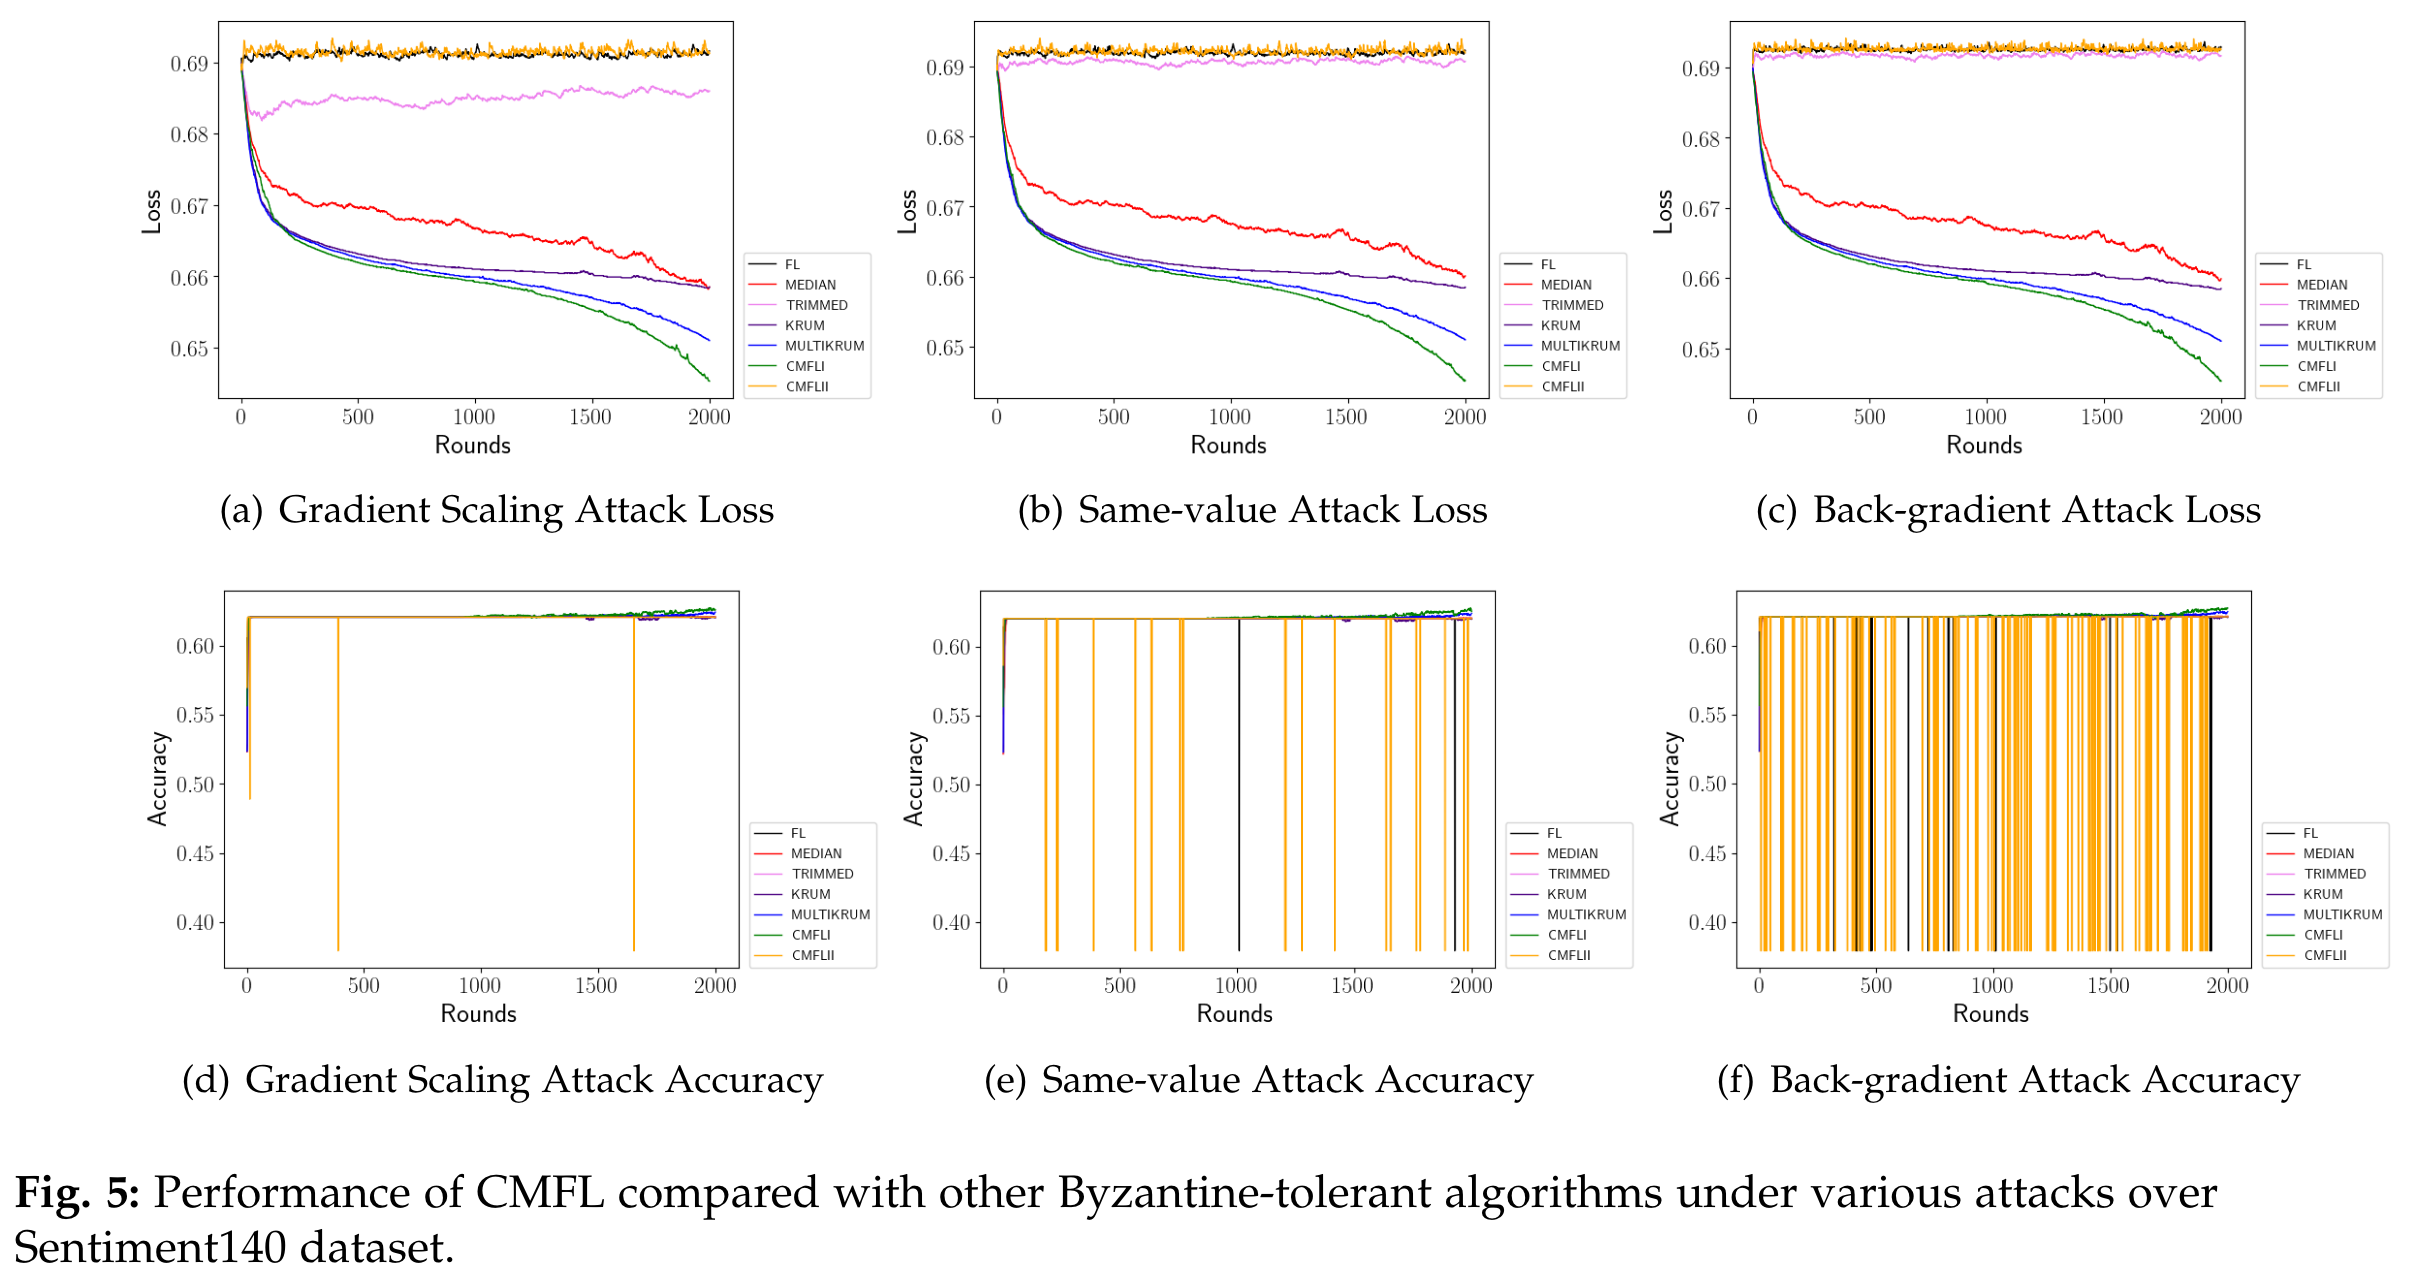
\includegraphics[width=0.78\textwidth]{images/exp_fig5}
\end{frame}

\begin{frame}{4.2 Robustness Comparative Experiment}{Result Analysis}
	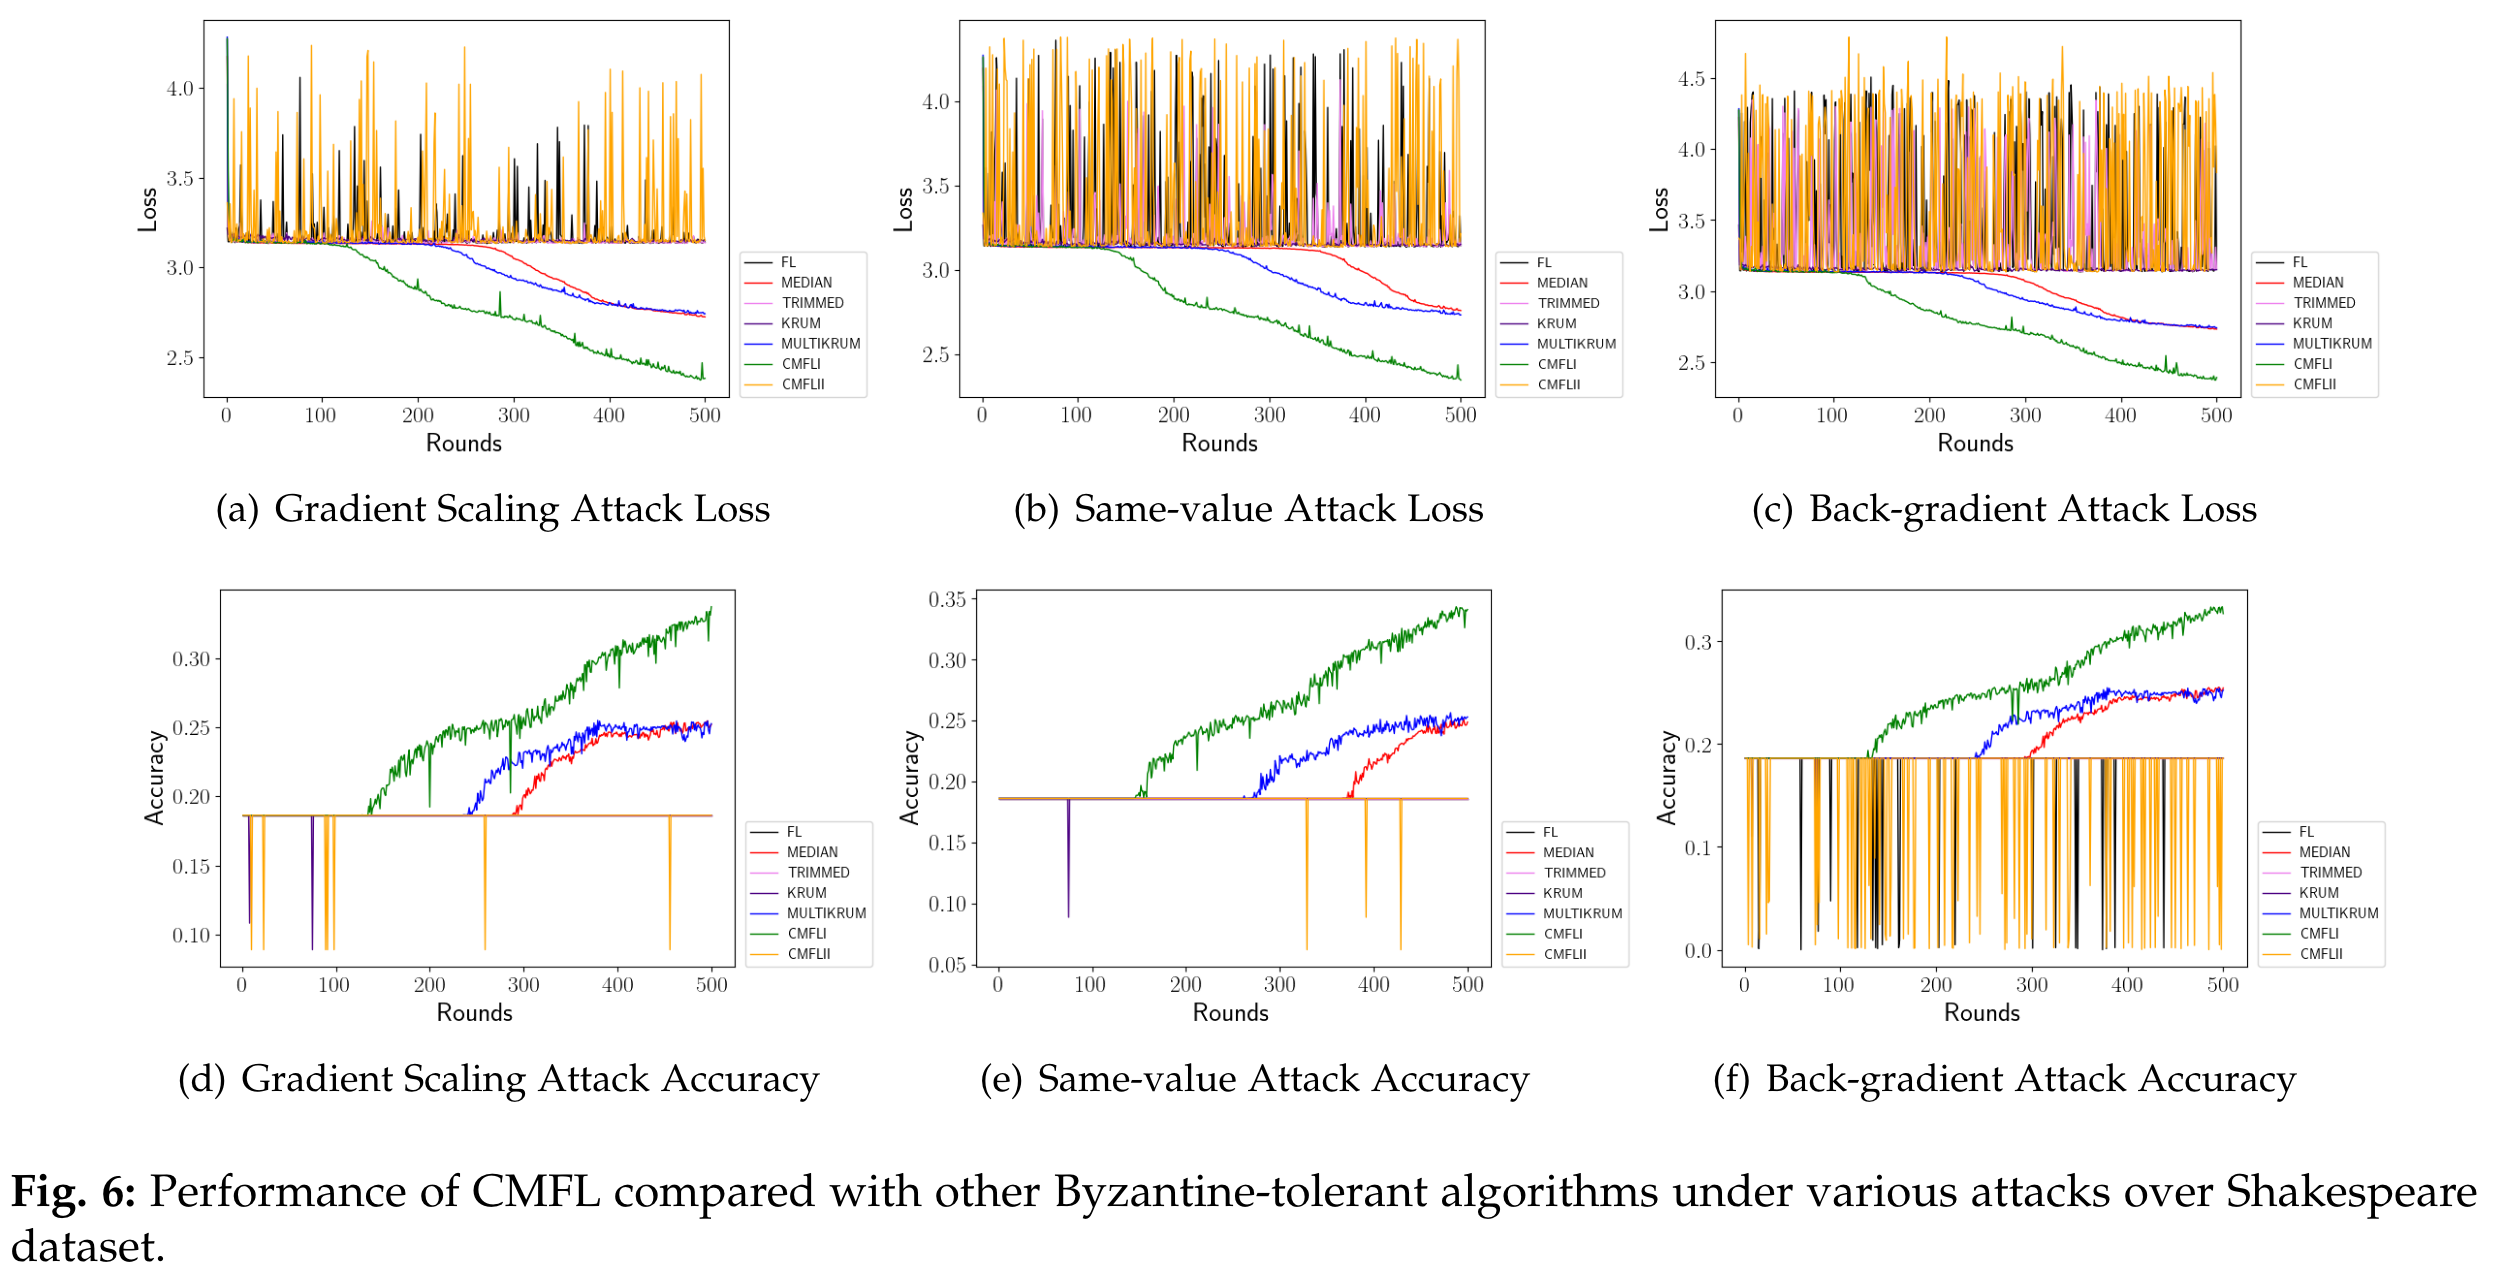
\includegraphics[width=0.78\textwidth]{images/exp_fig6}
\end{frame}

\section{Conclusions}

\begin{frame}{Conclusions}


\begin{itemize}
    \item 在本文中,我们提出了一个基于委员会机制的无服务器 FL 框架,它可以在考虑拜占庭攻击时确保鲁棒性。
    \item 此外,我们还为我们提出的框架提供了收敛保证。在理论分析的启发下,我们设计了选举和选择策略,使模型具有针对拜占庭攻击和恶意服务器问题的鲁棒性。
    \item 实验结果表明该模型优于典型的联邦学习和拜占庭容错模型,进一步验证了所提出框架的有效性和鲁棒性。
  \end{itemize}
\end{frame}



\backmatter

\end{document}
